\documentclass{scrartcl}
	%Aus dem LaTex Template der Universit�t Stuttgart
%------------------------------------------------
\usepackage[utf8]{inputenc}
\usepackage[T1]{fontenc}
\usepackage{cmap}
\usepackage[ngerman]{babel}
\usepackage{graphicx}
\usepackage[pdftex,hyperref,dvipsnames]{xcolor}
\usepackage{listings}
\usepackage[a4paper,lmargin={2cm},rmargin={2cm},tmargin={3.5cm},bmargin = {2.5cm},headheight = {4cm}]{geometry}
\usepackage{amsmath,amssymb,amstext,amsthm}
\usepackage[lined,algonl,boxed]{algorithm2e}
\usepackage{tikz}
\usepackage{hyperref}
\usepackage{url}
\usepackage[inline]{enumitem} % Erm�glicht �ndern der enum Item Zahlen
\usepackage[headsepline]{scrpage2} 
\usepackage{algorithmic} % F�r Pseudocode
\usepackage{ marvosym } % f�r Pfeil(e)
\usepackage{booktabs} % F�r die sch�neren Booktabs-Tabellen
\usepackage{tikz}
\usepackage{pdfpages}
\usepackage{blindtext}
\usepackage{scrextend}
\usepackage{natbib} % Yannis hat das importiert; TODO: nachfragen, zu was das gut ist
\pagestyle{scrheadings} 
\usetikzlibrary{automata,positioning}
	
	\begin{document}
		% Counter für das Blatt und die Aufgabennummer.
% Ersetze die Nummer des Übungsblattes und die Nummer der Aufgabe
% den Anforderungen entsprechend.
% Beachte:
% \setcounter{countername}{number}: Legt den Wert des Counters fest
% \stepcounter{countername}: Erhöht den Wert des Counters um 1.
\newcounter{sheetnr}
\setcounter{sheetnr}{6} % Nummer des Übungsblattes
\newcounter{exnum}
\setcounter{exnum}{1} % Nummer der Aufgabe

% Befehl für die Aufgabentitel
\newcommand{\exercise}[1]{\section*{Aufgabe \theexnum\stepcounter{exnum} #1}} % Befehl für Aufgabentitel

% Formatierung der Kopfzeile
% \ohead: Setzt rechten Teil der Kopfzeile mit
% Namen und Matrikelnummern aller Bearbeiter
\ohead{Yannis Blosch (3256958)\\
Lukas Heiland (3269754)\\
Nils Boike (3257520)}
% \chead{} kann mittleren Kopfzeilen Teil sezten
% \ihead: Setzt linken Teil der Kopfzeile mit
% Modulnamen, Semester und Übungsblattnummer
\ihead{Systemkonzepte und -programmierung\\
Wintersemester 2017/18\\
Blatt \thesheetnr}

		
		\section*{Aufgabe 2}
			\paragraph*{a)}
				\begin{itemize}
					\item $P_1$ wird von $P_2$ in eine Warteschlange eingereiht und $P_2$ geht in den kritischen Abschnitt, wenn $P_2$ fertig ist sendet er $"reply"$ an $P_1$
					\item $P_2$ sendet $"reply"$ an $P_1$ und wartet auf Antwort von $P_1$
					\item $P_2$ sendet $"reply"$ an $P_1$
				\end{itemize}
			
			\paragraph*{b)}
			$P_4 \rightarrow P_2 \rightarrow P_3 \rightarrow P_6 \rightarrow P_1 \rightarrow P_5$
			
			\paragraph*{c)}
			Beispiel Vorlesung "Nachrichtenaustausch" Seite 56
			
			\paragraph*{d)}
			!!!!!!!!!!!!!!!!!!!!!!!!!!!!!!
			
			\paragraph*{e)}
			Prozesse der Anzahl n, senden an jeweils n-1 prozesse Nachrichten x mal\\
			$(n \cdot (n-1)) \cdot x \Rightarrow n^2$\pagebreak
			
			
		\section*{Aufgabe 3}
			\paragraph*{a)}
				Wenn zum Zeitpunkt der Tokenverteilung mehrere Requests von Prozessen vorliegen, kann ein Prozess aushungern, da der Token zufällig zugeteilt wird.\\
				Bsp.: P1 und P2 requesten im Wechsel immer wieder, sodass P3 nie den Token bekommt (s.u.):\\[2em]
						
				\begin{figure}[h]
					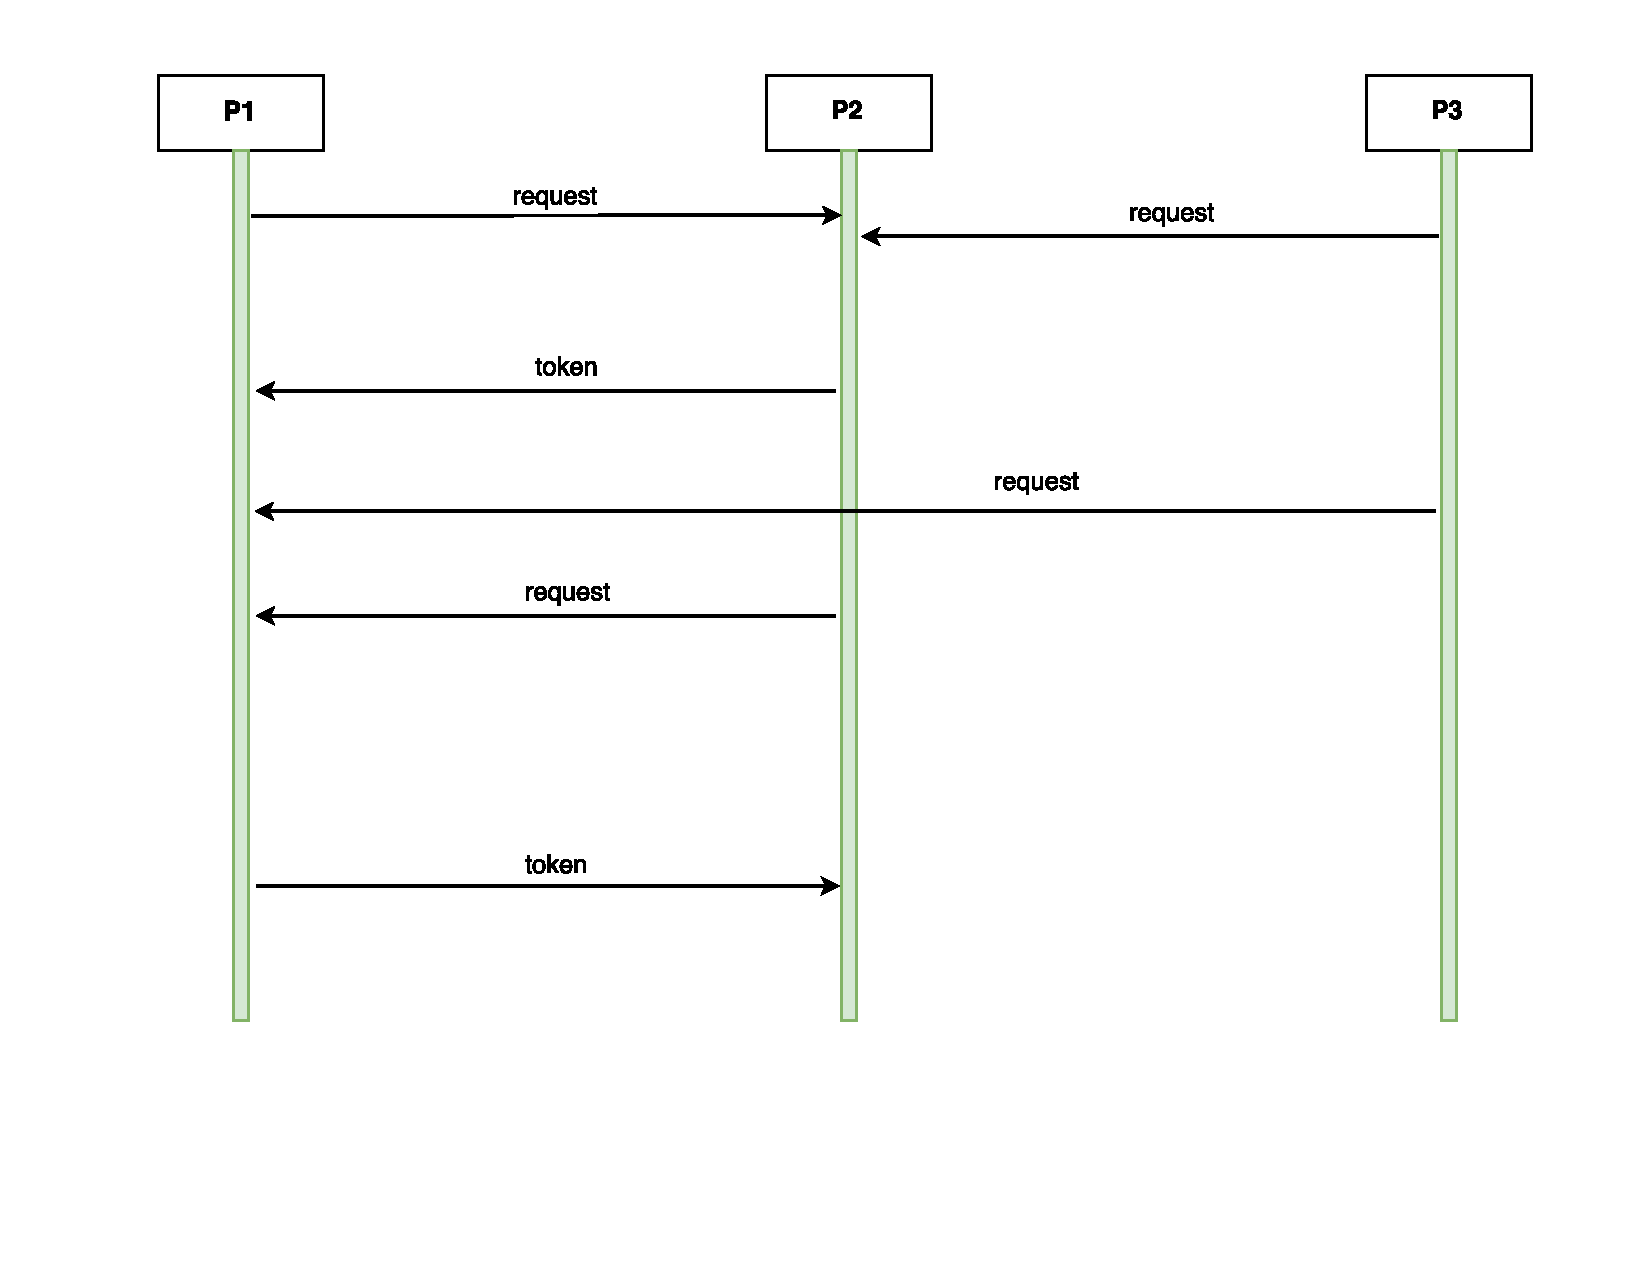
\includegraphics[scale=0.7]{aufgabe3a.pdf}
				\end{figure}
	\end{document}